\documentclass[tikz,border=10pt]{standalone}
\usetikzlibrary{mindmap}

\begin{document}
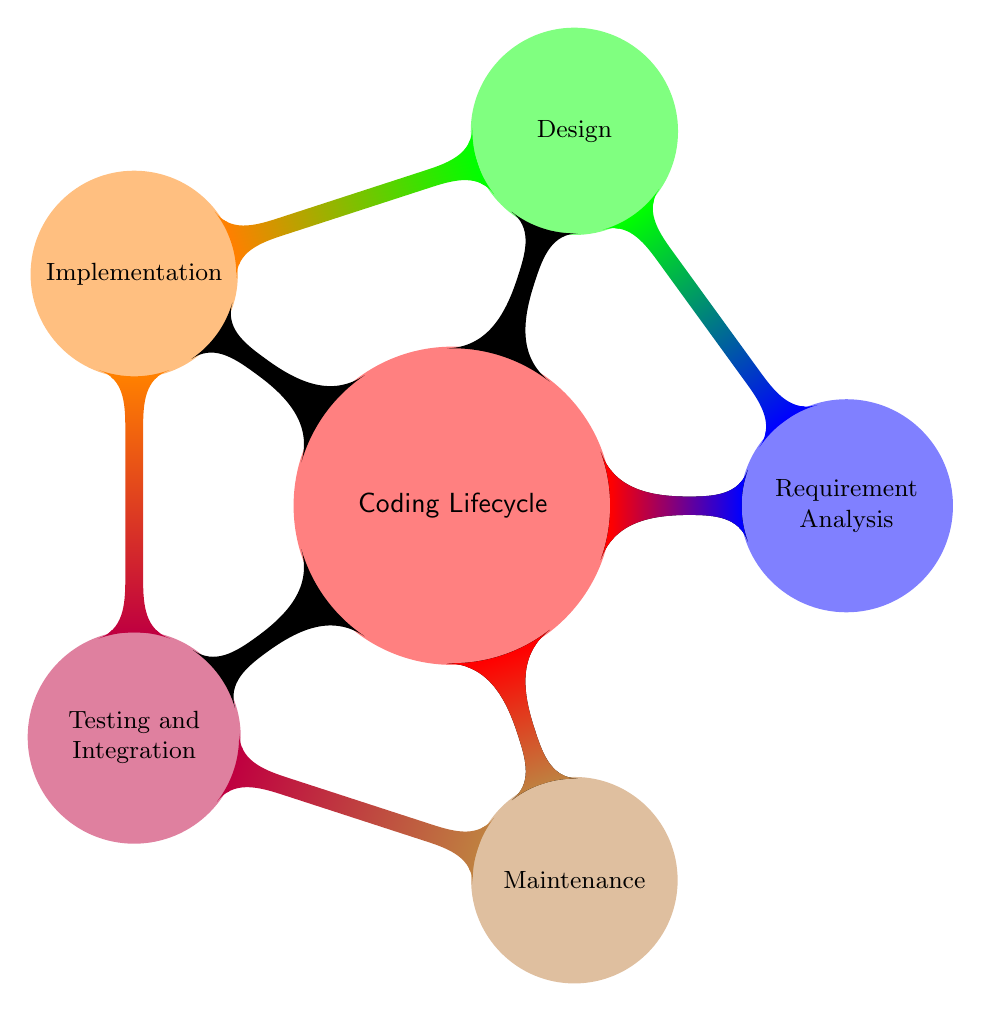
\begin{tikzpicture}[
    mindmap,
    concept/.append style={text width=2.5cm, align=center},
    font=\sffamily,
    every edge/.append style={decorate}
  ]
  \node [concept, concept color=red!50] (root) {Coding Lifecycle}
    child[grow=0] {node[concept, concept color=blue!50] (ra) {Requirement Analysis}}
    child[grow=72] {node[concept, concept color=green!50] (d) {Design}}
    child[grow=144] {node[concept, concept color=orange!50] (i) {Implementation}}
    child[grow=216] {node[concept, concept color=purple!50] (ti) {Testing and Integration}}
    child[grow=288] {node[concept, concept color=brown!50] (m) {Maintenance}};
  \path (root) to[circle connection bar switch color=from (red) to (blue)] (ra);
  \path (ra) to[circle connection bar switch color=from (blue) to (green)] (d);
  \path (d) to[circle connection bar switch color=from (green) to (orange)] (i);
  \path (i) to[circle connection bar switch color=from (orange) to (purple)] (ti);
  \path (ti) to[circle connection bar switch color=from (purple) to (brown)] (m);
  \path (m) to[circle connection bar switch color=from (brown) to (red)] (root);
\end{tikzpicture}
\end{document}